%% abtex2-modelo-trabalho-academico.tex, v-1.9.2 laurocesar
%% Copyright 2012-2014 by abnTeX2 group at http://abntex2.googlecode.com/ 
%%
%% This work may be distributed and/or modified under the
%% conditions of the LaTeX Project Public License, either version 1.3
%% of this license or (at your option) any later version.
%% The latest version of this license is in
%%   http://www.latex-project.org/lppl.txt
%% and version 1.3 or later is part of all distributions of LaTeX
%% version 2005/12/01 or later.
%%
%% This work has the LPPL maintenance status `maintained'.
%% 
%% The Current Maintainer of this work is the abnTeX2 team, led
%% by Lauro César Araujo. Further information are available on 
%% http://abntex2.googlecode.com/
%%
%% This work consists of the files abntex2-modelo-trabalho-academico.tex,
%% abntex2-modelo-include-comandos and abntex2-modelo-references.bib
%%

% ------------------------------------------------------------------------
% ------------------------------------------------------------------------
% abnTeX2: Modelo de Trabalho Academico (tese de doutorado, dissertacao de
% mestrado e trabalhos monograficos em geral) em conformidade com 
% ABNT NBR 14724:2011: Informacao e documentacao - Trabalhos academicos -
% Apresentacao
% ------------------------------------------------------------------------
% ------------------------------------------------------------------------

%-------------------------------------------------------------------------
% Modelo adaptado especificamente para o contexto do PPgSI-EACH-USP por 
% Marcelo Fantinato, com auxílio dos Professores Norton T. Roman, Helton
% H. Bíscaro e Sarajane M. Peres, em 2015, com muitos agradecimentos aos 
% criadores da classe e do modelo base.
%
% 20/06/2017: inclusão de "lista de quadros" com base no especificado em:
% https://github.com/abntex/abntex2/wiki/HowToCriarNovoAmbienteListing,
% de autoria de "Eduardo de Santana Medeiros Alexandre".
%
%-------------------------------------------------------------------------

\documentclass[
	% -- opções da classe memoir --
	12pt,				% tamanho da fonte
	% openright,			% capítulos começam em pág ímpar (insere página vazia caso preciso)
	oneside,			% para impressão apenas no anverso (apenas frente). Oposto a twoside
	a4paper,			% tamanho do papel. 
	% -- opções da classe abntex2 --
	%chapter=TITLE,		% títulos de capítulos convertidos em letras maiúsculas
	%section=TITLE,		% títulos de seções convertidos em letras maiúsculas
	%subsection=TITLE,	% títulos de subseções convertidos em letras maiúsculas
	%subsubsection=TITLE,% títulos de subsubseções convertidos em letras maiúsculas
	% -- opções do pacote babel --
	english,			% idioma adicional para hifenização
	%french,				% idioma adicional para hifenização
	%spanish,			% idioma adicional para hifenização
	brazil				% o último idioma é o principal do documento
	]{abntex2ppgsi}

% ---
% Pacotes básicos 
% ---
% \usepackage{lmodern}			% Usa a fonte Latin Modern			
% \usepackage[T1]{fontenc}		% Selecao de codigos de fonte.
\usepackage[utf8]{inputenc}		% Codificacao do documento (conversão automática dos acentos)

\usepackage{indentfirst}		% Indenta o primeiro parágrafo de cada seção.
\usepackage{color}				% Controle das cores
\usepackage{graphicx}			% Inclusão de gráficos
\usepackage{microtype} 			% para melhorias de justificação
\usepackage{pdfpages}     %para incluir pdf
\usepackage{algorithm}			%para ilustrações do tipo algoritmo
\usepackage{mdwlist}			%para itens com espaço padrão da abnt
\usepackage[noend]{algpseudocode}			%para ilustrações do tipo algoritmo
		
% ---
% Pacotes adicionais, usados apenas no âmbito do Modelo Canônico do abnteX2
% ---
\usepackage{lipsum}				% para geração de dummy text
% ---

% ---
% Pacotes de citações
% ---
\usepackage{hyperref}
\usepackage[brazilian,hyperpageref]{backref}	 % Paginas com as citações na bibl
\usepackage[alf,abnt-etal-list=0,abnt-etal-text=it]{abntex2cite}	% Citações padrão ABNT

% --- 
% CONFIGURAÇÕES DE PACOTES
% --- 

% ---
% Configurações do pacote backref
% Usado sem a opção hyperpageref de backref
\renewcommand{\backrefpagesname}{Citado na(s) página(s):~}
% Texto padrão antes do número das páginas
\renewcommand{\backref}{}
% Define os textos da citação
\renewcommand*{\backrefalt}[4]{
	\ifcase #1 %
		Nenhuma citação no texto.%
	\or
		Citado na página #2.%
	\else
		Citado #1 vezes nas páginas #2.%
	\fi}%
% ---

\instituicao{
	UNIVERSIDADE DE SÃO PAULO
	\par
	ESCOLA DE ARTES, CIÊNCIAS E HUMANIDADES
	\par
	PROGRAMA DE GRADUAÇÃO EM SISTEMAS DE INFORMAÇÃO}

\titulo{Ensaio sobre o documentário \emph{Revolution OS}}

\autor{\uppercase{Felipe Mateos Castro de Souza}}

\local{São Paulo}

\data{2023}

\orientador{Profa. Gisele da Silva Craveiro}
\coorientador{Prof. Wagner Luiz Taques da Rocha}

\tipotrabalho{Ensaio}

\preambulo{
Ensaio apresentada à Escola de Artes, Ciências e Humanidades da Universidade de São Paulo como componente do método avaliativo da Disciplina ACH3778 - Governo Aberto.}

\definecolor{blue}{RGB}{41,5,195}

% informações do PDF
\makeatletter
\hypersetup{
     	%pagebackref=true,
		pdftitle={\@title}, 
		pdfauthor={\@author},
    	pdfsubject={\imprimirpreambulo},
	    pdfcreator={laTeX com abnTeX2 adaptado para o PPgSI-EACH-USP},
		pdfkeywords={abnt}{latex}{abntex}{abntex2ppgsi}{qualificação de mestrado}{dissertação de mestrado}{qualificação de doutorado}{tese de doutorado}{ppgsi}, 
		colorlinks=true,       		% false: boxed links; true: colored links
    	linkcolor=blue,          	% color of internal links
    	citecolor=blue,        		% color of links to bibliography
    	filecolor=magenta,      		% color of file links
		urlcolor=blue,
		bookmarksdepth=4
}
\makeatother

\setlength{\parindent}{1.25cm}

\setlength{\parskip}{0cm} 
\renewcommand{\baselinestretch}{1.5}

\makeindex

  \clubpenalty10000
  \widowpenalty10000
  \displaywidowpenalty10000

\begin{document}

\frenchspacing 

\imprimircapa

\imprimirfolhaderosto*

\setlength{\absparsep}{18pt} 

\pdfbookmark[0]{\listfigurename}{lof}
\listoffigures*
\cleardoublepage

\begin{siglas}
  \item[GNU] General Public License
\end{siglas}

\pdfbookmark[0]{\contentsname}{toc}
\tableofcontents*
\cleardoublepage



% ----------------------------------------------------------
% ELEMENTOS TEXTUAIS
% ----------------------------------------------------------
\textual

\chapter{Disputa entre os movimentos\emph{Open} e \emph{Free}}
\section{Considerações inciais}
Para entender mais sobre o assunto, além de assistir ao documetário, também consultei colegas mais experientes, bem como fiz uso de uma bibliografia adicional.

\section{Introdução}
O documentário, publicado no canal \emph{\citeonline{revolutionOS}}, entitulado ``Revolution OS" narra a história do surgimento e crescimento do movimento do software livre e de código aberto, e apresenta argumentos convincentes sobre a superioridade do modelo de código aberto em comparação com o modelo de software livre. Embora ambos os modelos tenham objetivos semelhantes, que são promover a liberdade de acesso e uso de software, há diferenças fundamentais que os distinguem.



Uma forma simples de ilustrar seria com o exemplo de duas licenças amplamente usadas, sendo estas a GNU GPL e a MIT Licence.

\section{Diferença entre GNU GPL e MIT Licence}
Segundo as fontes: \citeonline{snyk} e o \citeonline{chatgpt}, a Licença Pública Geral GNU (GPL) e a Licença MIT são duas licenças de software livre que diferem em termos de seus objetivos e requisitos.

A GPL é uma licença copyleft que garante que o software livre permaneça livre e aberto, mesmo quando é modificado e redistribuído. A GPL exige que quaisquer trabalhos derivados sejam licenciados sob os mesmos termos da GPL, o que significa que os usuários têm o direito de usar, copiar, modificar e redistribuir o software livremente, mas devem compartilhar essas liberdades com outros usuários.

Por outro lado, a Licença MIT é uma licença permissiva que permite que os usuários usem, copiem, modifiquem e redistribuam o software livremente, sem restrições. A Licença MIT é uma licença de "cola" permissiva, o que significa que os usuários podem incluir o código sob a licença MIT em software proprietário, sem a necessidade de compartilhar o código-fonte do software proprietário.

\begin{figure}[H]% H manda colocar exatamente nessa posição no texto (relativa aos parágrafos anterior e posterior)
	\centering
 	  \caption{Diagrama contendo a relação entre Aberto (\emph{Open}) e Livre (\emph{Free})}
		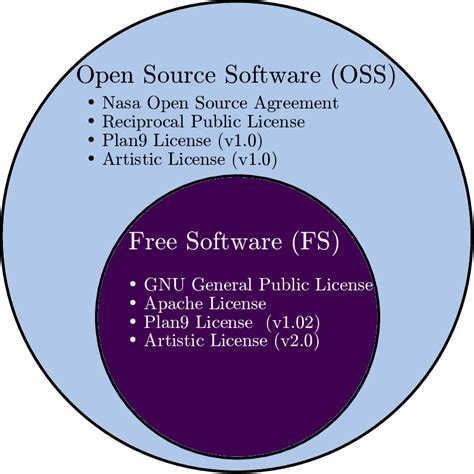
\includegraphics[scale=0.5]{euler.jpg}
	\label{fig:euler}
  \source{\citeonline{mostfreeware}}
\end{figure}


\section{Vantagens do modelo Aberto sobre o Livre}
 
Uma das principais vantagens do modelo de código aberto é a transparência e a colaboração entre desenvolvedores. No modelo de software livre, o código fonte é disponibilizado sem restrições, mas não necessariamente é compartilhado e melhorado de forma colaborativa pela comunidade de desenvolvedores. Por outro lado, no modelo de código aberto, o código fonte é não só disponibilizado, mas também é aberto à contribuição de qualquer pessoa, permitindo que a comunidade de desenvolvedores trabalhe em conjunto para melhorar e aprimorar o software.

Além disso, o modelo de código aberto incentiva a inovação e a competitividade saudável entre as empresas, ao invés de limitar o acesso ao software por meio de licenças restritivas. Empresas que utilizam e contribuem para projetos de código aberto podem ter vantagens competitivas, ao mesmo tempo em que ajudam a melhorar a qualidade do software e a avançar a tecnologia em geral. Isso contrasta com o modelo de software livre, em que o acesso ao código fonte é limitado a uma comunidade específica de desenvolvedores e usuários, reduzindo as oportunidades de inovação e colaboração.

Outra vantagem do modelo de código aberto é a sua flexibilidade em relação aos usuários finais. Os usuários têm a liberdade de modificar e personalizar o software para atender às suas necessidades específicas, sem ter que pagar por licenças ou solicitar permissão aos desenvolvedores. Isso permite que os usuários tenham mais controle sobre o software que utilizam, e também promove uma cultura de compartilhamento de conhecimento e soluções personalizadas.

\section{Conclusão}
 
Por fim, o modelo de código aberto tem uma vantagem importante em termos de segurança. Como o código fonte é aberto, a comunidade de desenvolvedores pode detectar e corrigir rapidamente problemas de segurança, garantindo que o software seja seguro e confiável. Isso contrasta com o modelo de software proprietário, em que os usuários não têm acesso ao código fonte e dependem exclusivamente do fabricante do software para corrigir vulnerabilidades.

\begin{figure}[H]
	\centering
		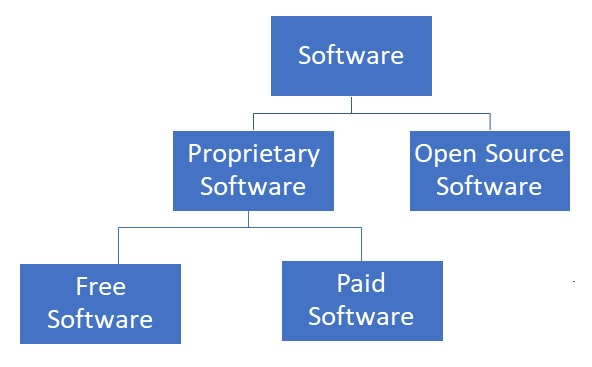
\includegraphics{tree.jpg}
	\label{fig:tree}
  \source{\citeonline{mostfreeware}}
\end{figure}

Em conclusão, embora ambos os modelos de software livre e código aberto tenham seus méritos, o modelo de código aberto é superior em termos de transparência, colaboração, inovação, flexibilidade e segurança. O modelo de código aberto promove uma cultura de compartilhamento de conhecimento e soluções personalizadas, permitindo que a tecnologia avance de forma mais rápida e eficiente. Portanto, para aqueles que buscam a liberdade e o controle sobre o software que utilizam, o modelo de código aberto é a melhor escolha.

\postextual

\bibliography{referencias}

\end{document}
